\chapter{IUGONETプロジェクトとメタデータ・データベース}

\section{はじめに}
 このドキュメントは、主にIUGONETプロジェクト外部からメタデータを提供して頂く際に、メタデータ作成を
担当される方向けに、
\begin{itemize}
\item メタデータ作成の手順、
\item メタデータ登録の方法、
\end{itemize}
をまとめたドキュメントです。メタデータ作成・登録の際に、この文章に
目を通して頂き、所定のフォーマットに沿ったメタデータを、効率よく作成・
登録して頂ければ幸いです。

\section{IUGONETプロジェクト}
 超高層大気長期変動の全球地上ネットワーク観測・研究(IUGONET: Inter-university Upper atmosphere Global Observation NETwork)
\footnote{http://www.iugonet.org/}は、平成21年度より6年計画としてスタートした大学間連携プロジェクトです。
このプロジェクトでは、国立極地研究所(宙空圏研究グループ)、東北大学(理学研究科地球物理学専攻太陽惑星空間物理学講座、惑星プラズマ・大気研究センター)、
名古屋大学(太陽地球環境研究所)、京都大学(生存圏研究所、大学院理学研究科附属地磁気世界資料解析センター、
大学院理学研究科附属天文台)、および九州大学(国際宇宙天気科学・教育センター、旧:宙空環境研究センター)
の5機関7組織が連携し、各々の研究機関が世界各地において実施している超高層大気の地上観測を有機的にリンクさせることにより、
全球地上ネットワーク観測網を形成し、それを利用した超高層大気の長期変動に関する研究を行うことを目的としています。\par

\section{メタデータ・データベース}
 IUGONET参加各機関において、個別に公開されている超高層大気の地上観測に関する様々なデータを、より効率的に流通させる為に、
1. 観測データからメタデータを抽出し、2. それらをデータベース化することにより、
様々な分野の研究者間で観測データに関する情報を共有するシステム、すなわちメタデータ・データベースを構築しています
(図\ref{mdb1.eps}, 図\ref{mdb2.eps}, 図\ref{mdb3.eps})。
このメタデータ・データベースはIUGONET参加機関のみならず、インターネットを
通して研究者コミュニティ全体に公開されています
\footnote{http://search.iugonet.org/iugonet/}。

\begin{figure}[H]
\begin{center}
\fbox{
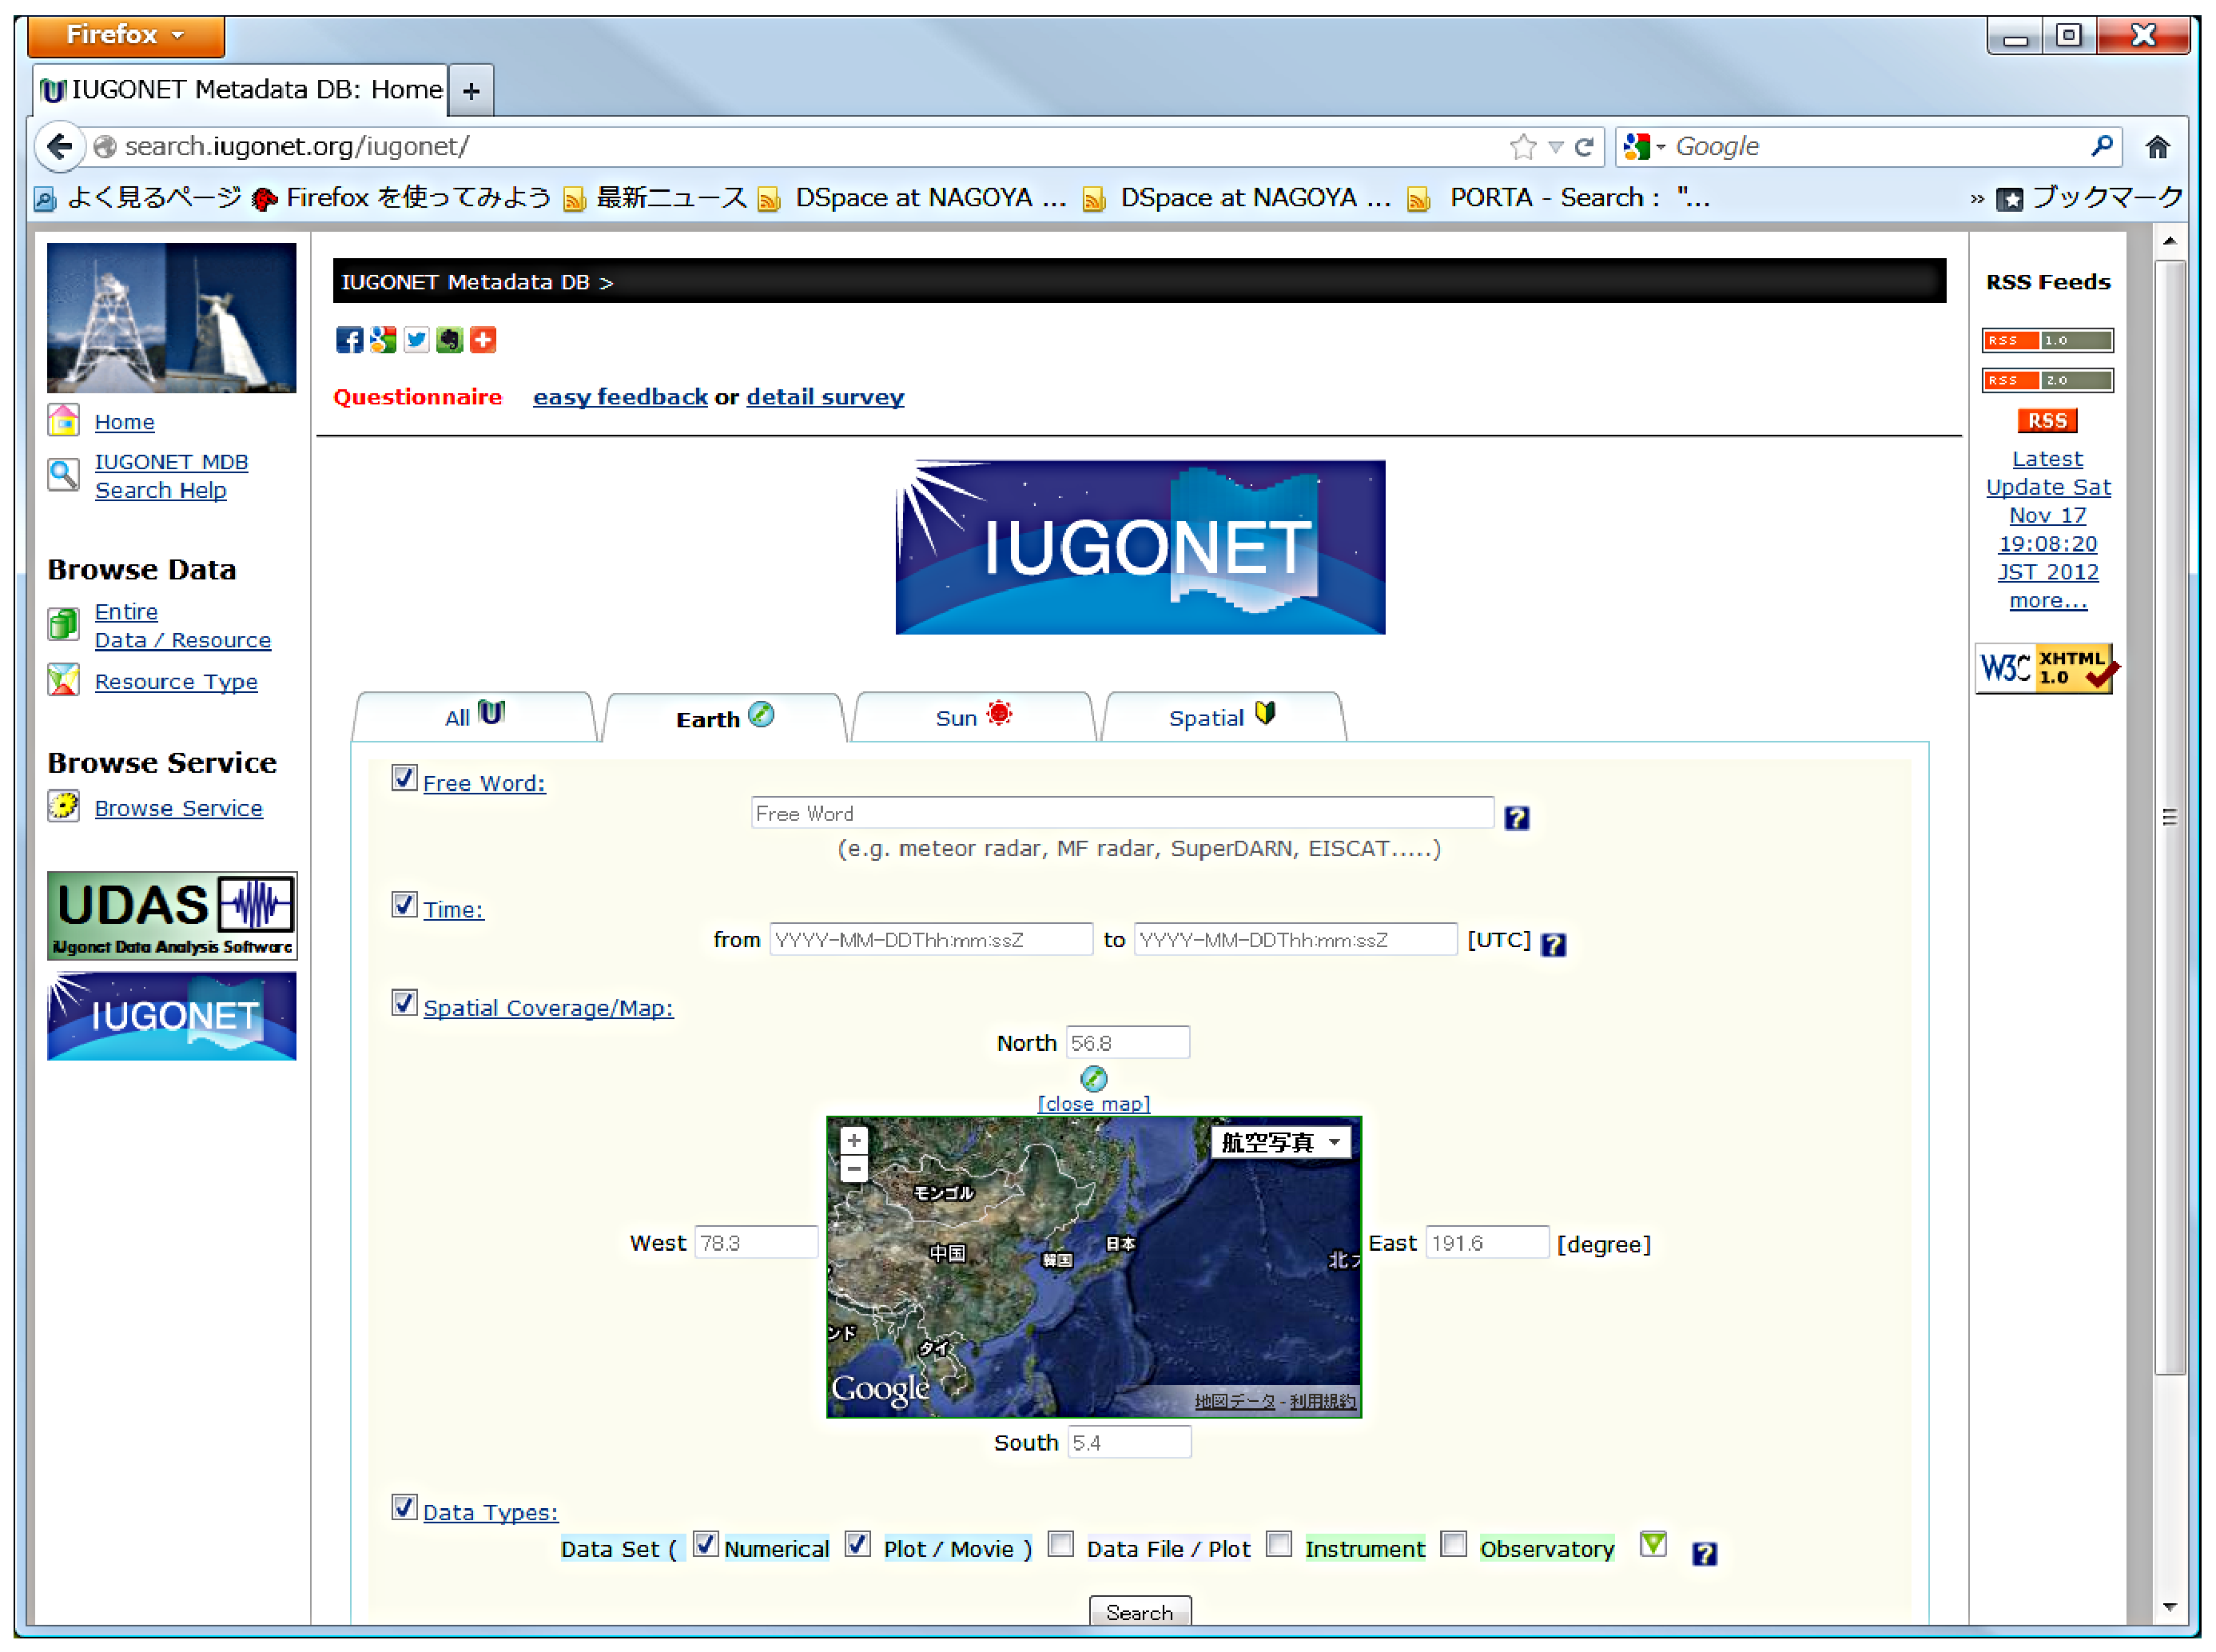
\includegraphics[width=12cm]{images/mdb1.eps}
}
\caption{メタデータ・データベースのスナップショットを示します。
フリーワード検索、時刻検索、領域検索が可能です。1クエリーで、
様々な観測データのメタデータを検索可能です。デフォルト設定では、
データセットのみを検索対象とする様に、チェックボックスが設定されています。このチェックボックスによる
検索対象の切り替えを駆使することにより、1データファイルに紐づいた、より粒度の細かいメタ
データ検索や、観測所情報、計測器情報などを検索することが可能になります。}
\label{mdb1.eps}
\end{center}
\end{figure}

\begin{figure}[H]
\begin{center}
\fbox{
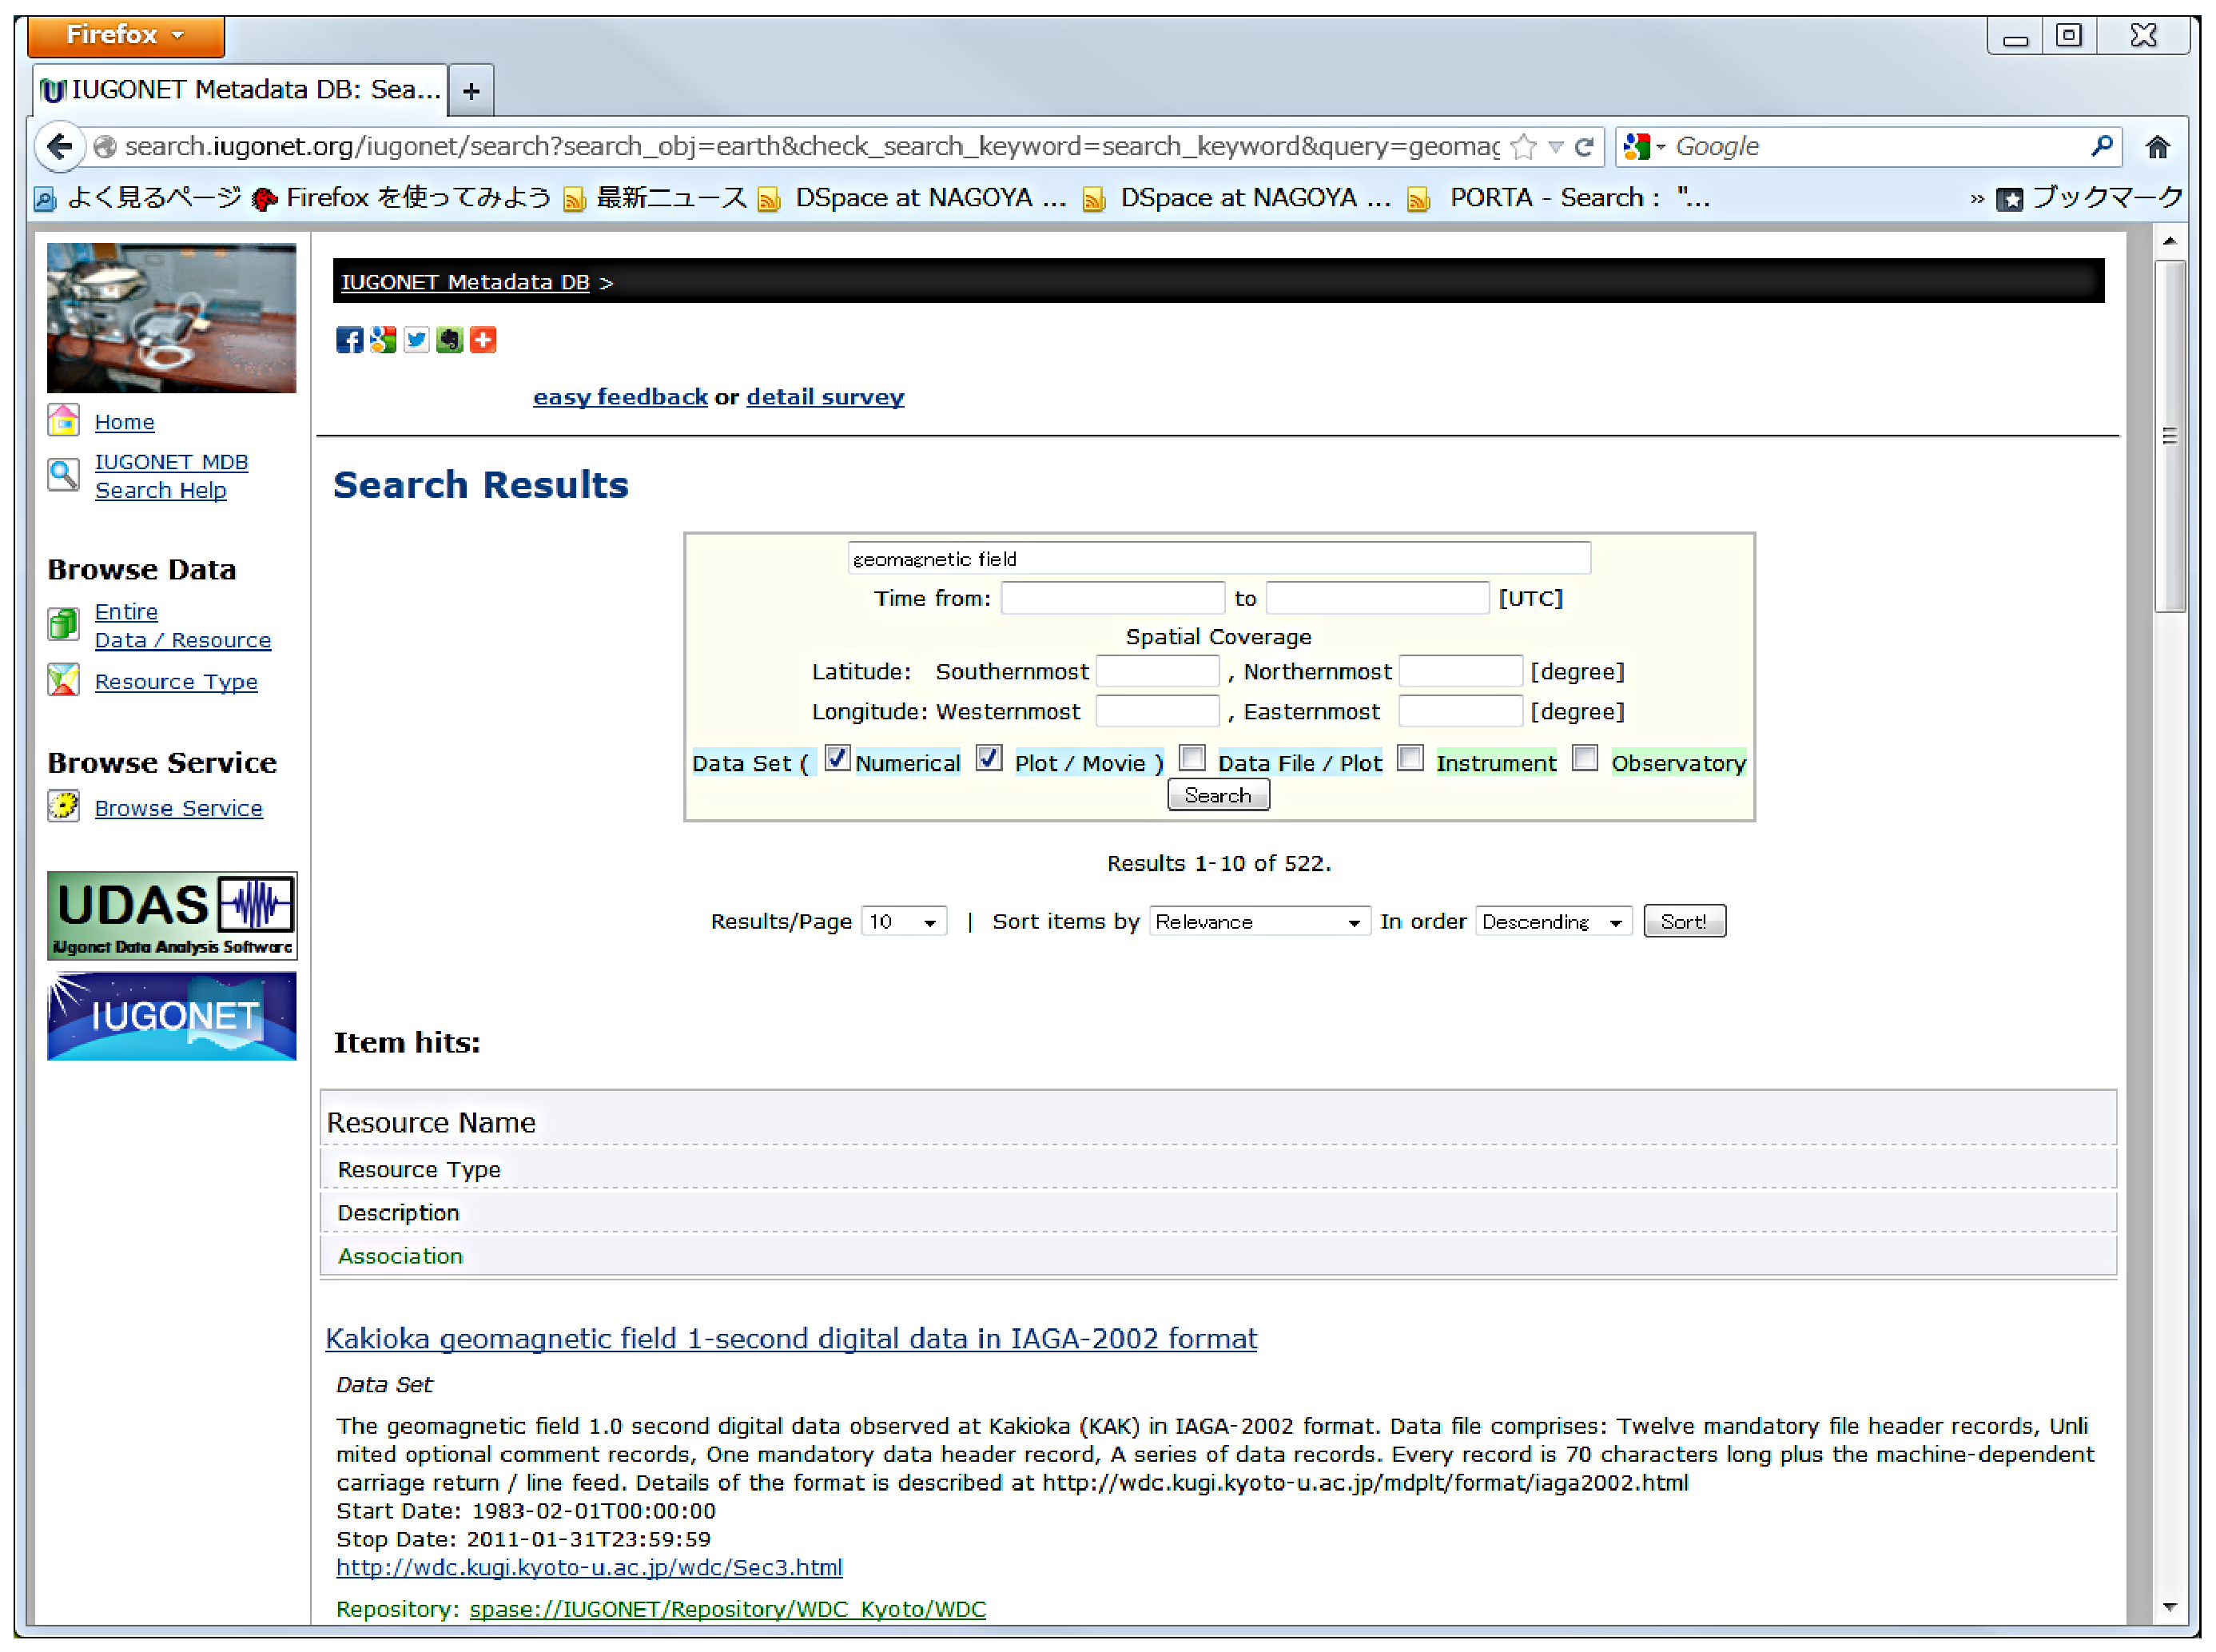
\includegraphics[width=12cm]{images/mdb2.eps}
}
\caption{フリーワード"geomagnetic field"で検索した際の検索結果一覧画面を示します。
検索結果一覧から、さらに絞込みをかけることが可能です。検索結果一覧からリンクをクリック
することにより、図\ref{mdb3.eps}に示した様なメタデータの詳細を閲覧することが可能です。}
\label{mdb2.eps}
\end{center}
\end{figure}

\begin{figure}[H]
\begin{center}
\fbox{
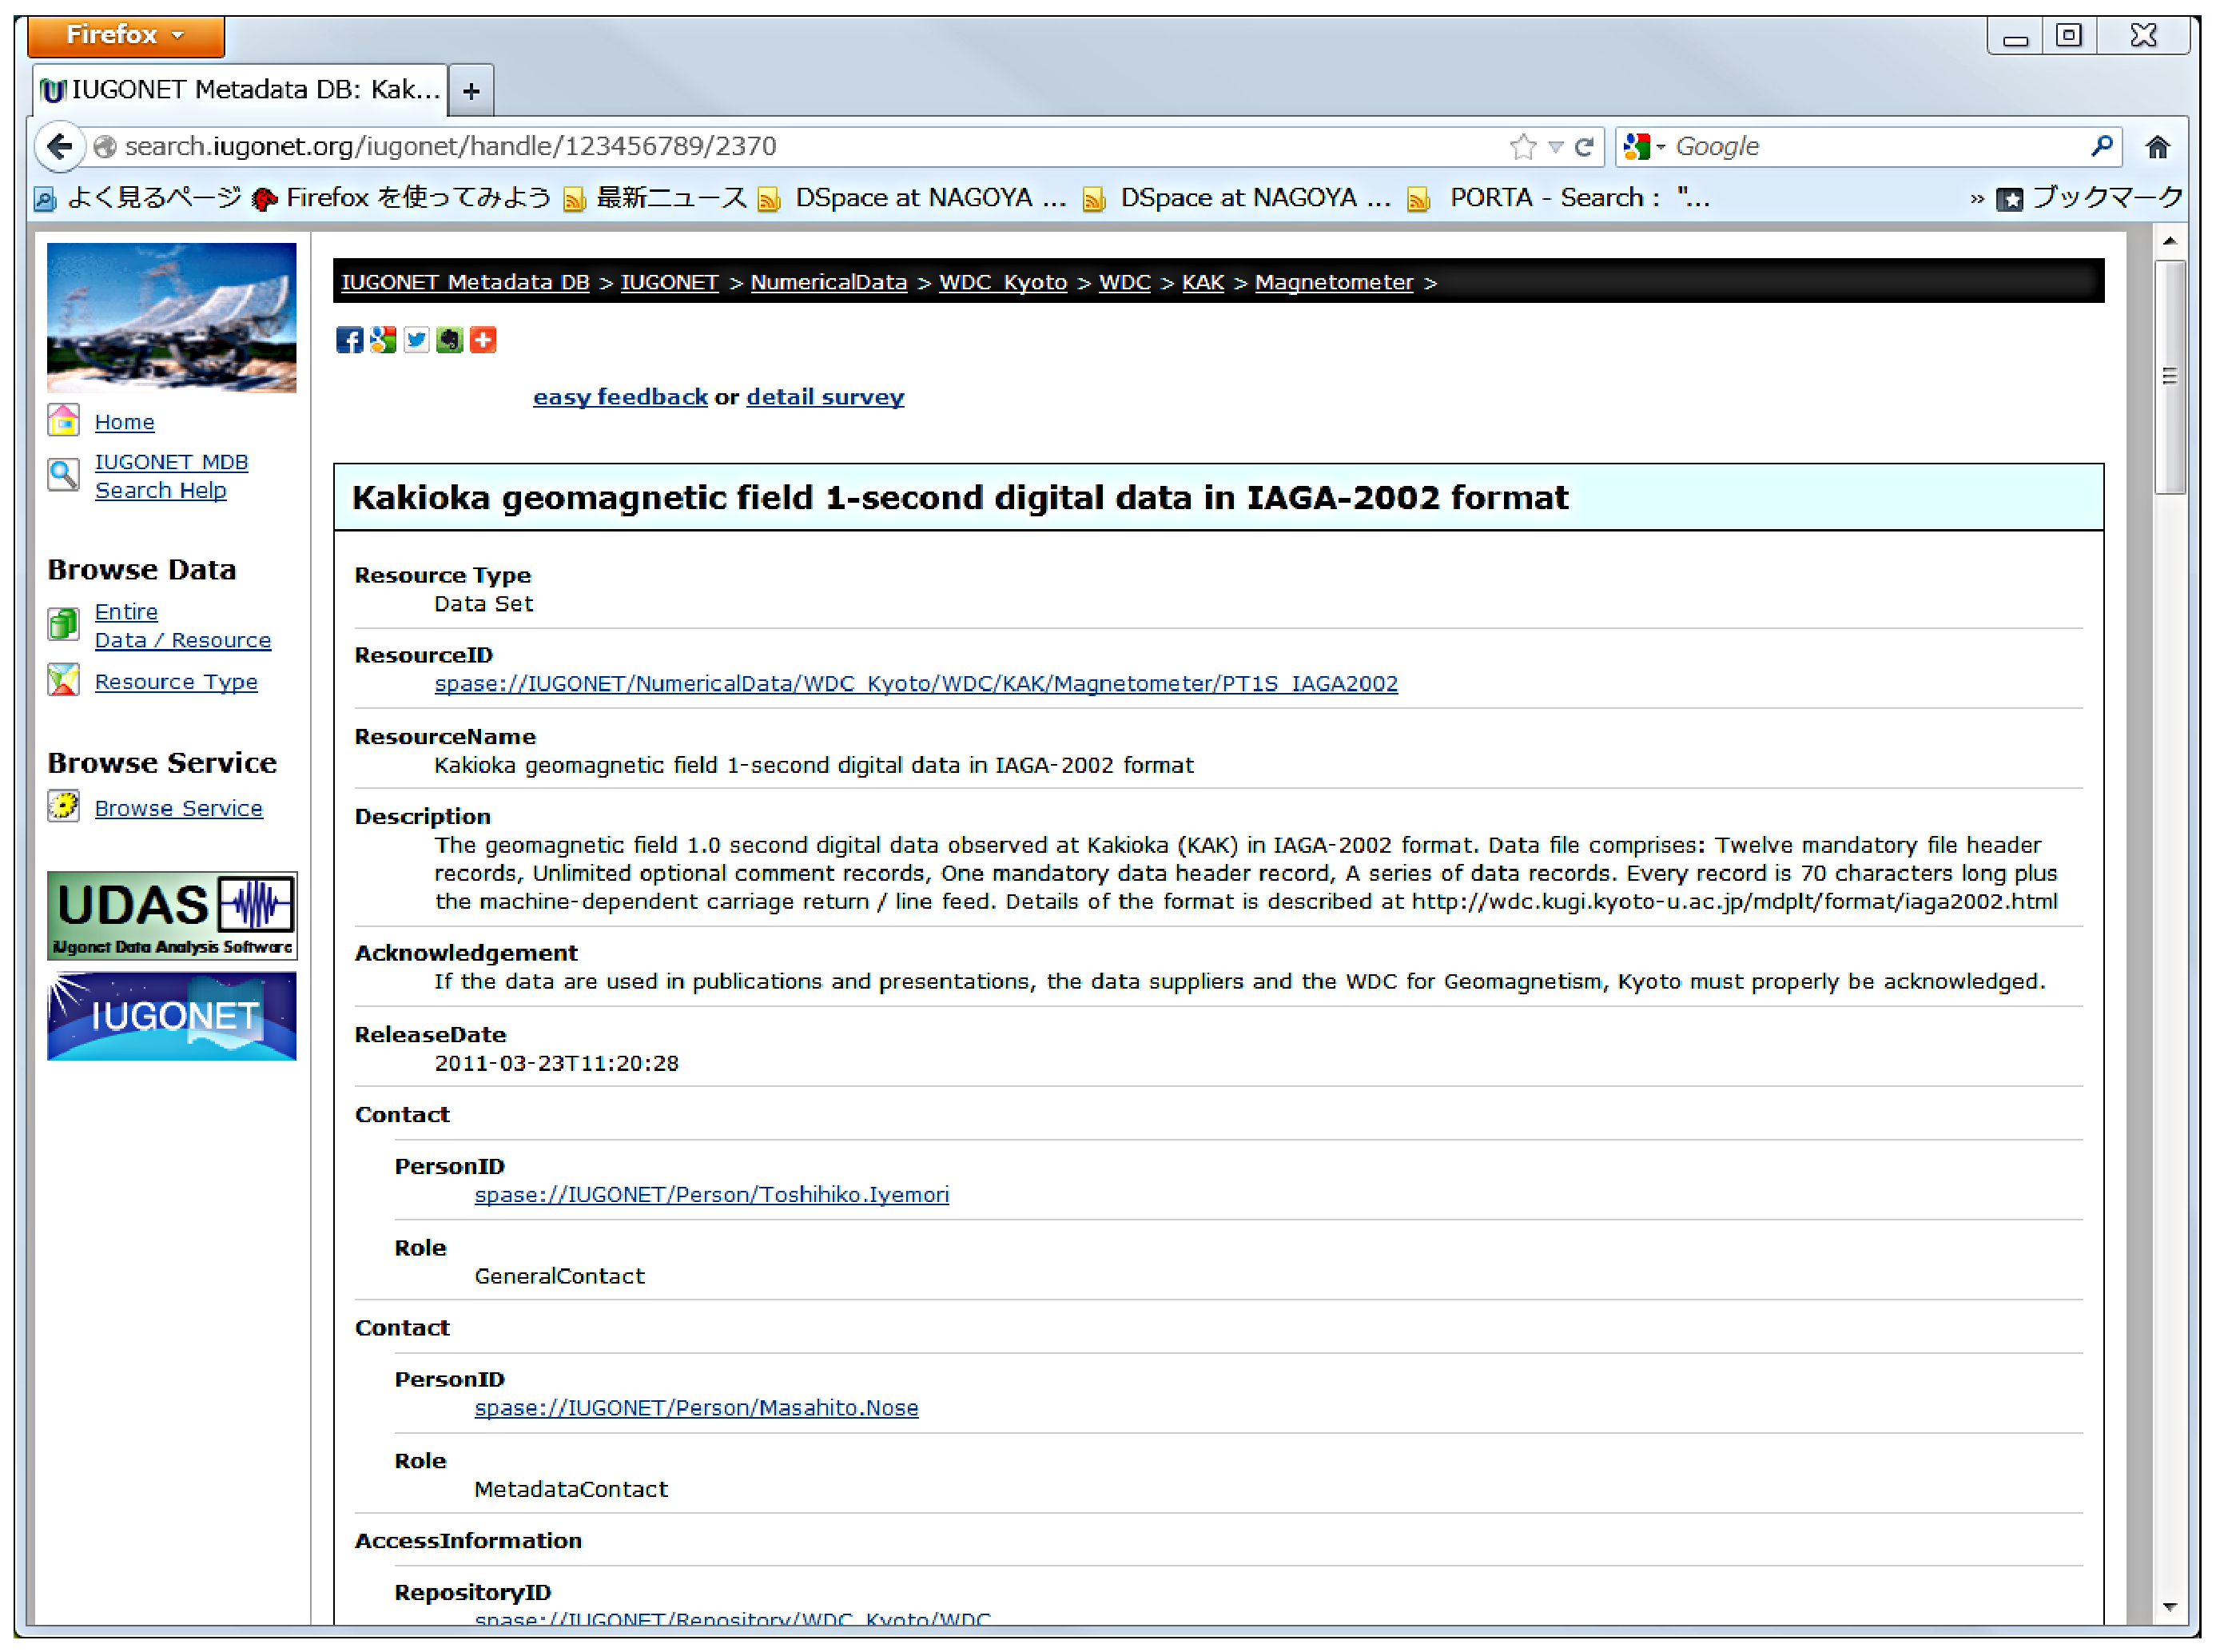
\includegraphics[width=12cm]{images/mdb3.eps}
}
\caption{メタデータの詳細表示の例として、kakioka geomagnetic field 1-second digital data in IAGA-formatに
関するメタデータを示します。AccessInformationに、このデータセットを
公開しているサイトへのリンクが張られています。}
\label{mdb3.eps}
\end{center}
\end{figure}

\section{メタデータ}
\begin{itemize}
\item 登録したデータがIUGONETメタデータDBでの検索でヒットするようになる、
\item データの存在を知らない研究者に、データの存在を知ってもらえる、
\end{itemize}

IUGONETプロジェクトでは、IUGONET参加機関以外の大学・研究機関からの、
メタデータ提供を歓迎します。IUGONETメタデータ・データベースが、様々な
研究機関から提供されるメタデータによって充実すれば、既に登録された
メタデータの付加価値も上がる可能性があります。

既にIUGONETメタデータ・データベースに登録されているメタデータと、
1クエリーで横断的に検索される可能性が高まり、学際的研究に発展する
必要があります。